\documentclass[a4paper]{article}
\title{MA2 - Nekonečně mnoho sedlových bodů}
\author{Tommy Chu}
\date{}

\usepackage[czech]{babel}
\usepackage[utf8]{inputenc}
\usepackage[T1]{fontenc}
\usepackage{graphicx}
\usepackage{amsmath}
\usepackage{amsthm}
\usepackage{amssymb}
\usepackage{subfiles}
\usepackage{hyperref}
\usepackage{geometry}
\usepackage{mathtools}
\usepackage{algpseudocode}
\usepackage{algorithm}
\usepackage{physics}
\usepackage{dsfont}
\usepackage{bm}
\usepackage{bbm}
\usepackage{float}
\usepackage{enumitem}
\usepackage{multirow}
\usepackage{tikz}
\usepackage{tikz-cd}
\usepackage{pgfplots}
\usepackage{lmodern}
\usepackage{import}
\usepackage{microtype}
\usepackage{fancyhdr}
\usepackage{parskip}
\usepackage{titling}
\usepackage{bookmark}

\graphicspath{ {./images/} }
\pgfplotsset{compat=1.18}
\microtypesetup{
    protrusion=true,
    activate={true,nocompatibility},
    final,
    tracking=true,
    kerning=true,
    spacing=true,
    factor=1100,
}

\relpenalty   = 10000
\binoppenalty = 10000

\setlength{\droptitle}{-5em}

\begin{document}
\maketitle

\section*{Zadání}

Najděte funkci tří proměnných, která má \textbf{(1)} nekonečně mnoho bodů s nulovým gradientem, z nichž ale \textbf{(2)} žádný není extrém.

\subsection*{Řešení}

Uvažujme hladkou funkci $f \colon \mathbb{R}^3 \rightarrow \mathbb{R}$:
\[
    f(x,y,z) = x^3.
\]

Takto definovaná funkce splňuje všechny podmínky v zadání.

\paragraph*{Důkaz:}

Gradient $f$ je nulový v bodech ${ S = \bigl\{ (0,y,z) \mid y,z \in \mathbb{R} \bigr\} }$:
\[
    \nabla f(x,y,z) = \big(3x^2,\, 0,\, 0\big) \ \Rightarrow \
    \forall \vb x \in S \colon \nabla f(\vb x) = \theta.
\]

\textbf{(1)} Bodů s nulovým gradientem je nekonečně mnoho:
\[
    |S| = |\mathbb{R}^2|.
\]

\textbf{(2)} Funkce nemá extrém v žádném bodě $S$. Na okolí každého bodu ${(0,y,z) \in S}$ platí, že ${f(x,y,z) = x^3}$ je kladné pro ${x>0}$ a záporné pro ${x<0}$.

Graf této funkce je vykreslen na následujícím \emph{3D contour plot}, kde funkční hodnota je znázorněna barvou.
Množinu sedlových bodů $S$ tvoří rovina ${x=0}$.
\qed

\begin{center}
    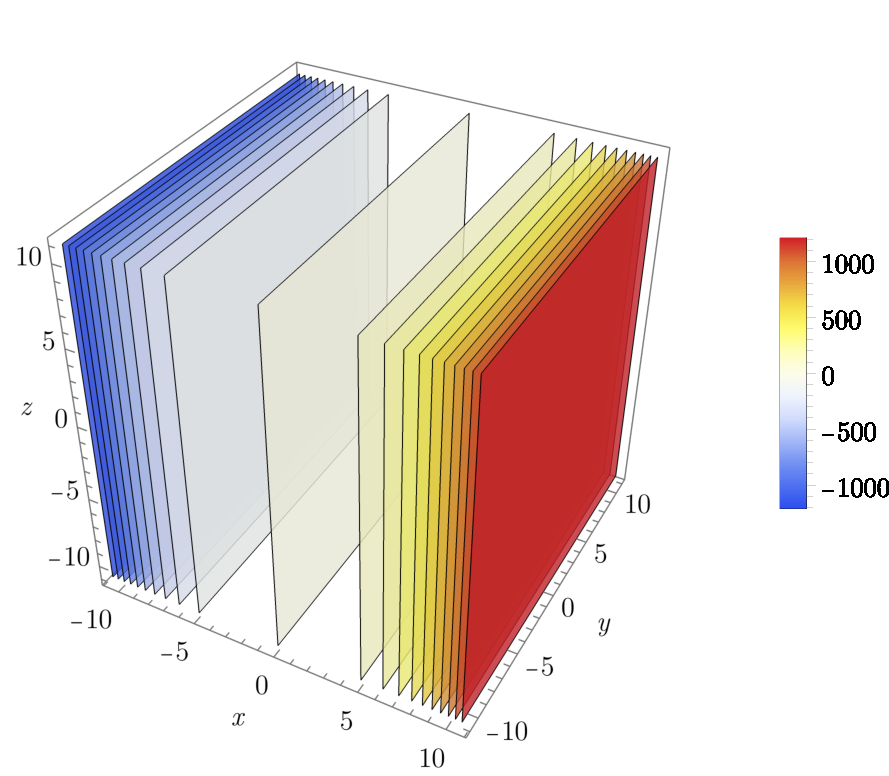
\includegraphics[width=8cm]{f.pdf}
\end{center}

\end{document}
